\documentclass[aspectratio=169]{beamer}

% Theme and color scheme
\usetheme{metropolis}
\usecolortheme{default}
\setbeamertemplate{navigation symbols}{}

% Packages
\usepackage[utf8]{inputenc}
\usepackage{amsmath,amssymb,amsfonts}
\usepackage{pifont} % for checkmarks
\usepackage{graphicx}
\usepackage{booktabs}
\usepackage{array}
\usepackage{xcolor}
\usepackage{tikz}
\usetikzlibrary{shapes,arrows}
\usepackage{pgfplots}
\pgfplotsset{compat=1.9}

% Custom colors for consistency
\definecolor{ifacblue}{RGB}{0,82,147}
\definecolor{ifacgray}{RGB}{128,128,128}
\definecolor{successgreen}{RGB}{46,125,50}
\definecolor{warningorange}{RGB}{255,152,0}
\definecolor{errorred}{RGB}{211,47,47}

% Tikz styles
\tikzstyle{block} = [rectangle, draw, fill=ifacblue!20, text width=12em, text centered, rounded corners, minimum height=3em]
\tikzstyle{arrow} = [thick,->,>=stealth]

% Set primary color
\setbeamercolor{frametitle}{bg=ifacblue,fg=white}
\setbeamercolor{progress bar}{fg=ifacblue}

% Title page information
\title{ODEParameterEstimation.jl: \\ Robust Parameter Estimation for ODEs}
\author{Oren Bassik}
\institute{JuliaCon 2025}
\date{\today}

\begin{document}

% Slide 1: Title
\begin{frame}
  \titlepage
\end{frame}

% Slide 2: The Big Picture
\begin{frame}{The Big Picture: What is ODEParameterEstimation.jl?}
    \begin{columns}[T]
        \begin{column}{0.5\textwidth}
            \Large
            Many real-world systems are described by ODEs, but we often don't know the parameters.
            \vspace{1em}
            
            \normalsize
            \texttt{ODEParameterEstimation.jl} is a toolbox for discovering these unknown parameters directly from data.
            
        \end{column}
        \begin{column}{0.5\textwidth}
            \centering
            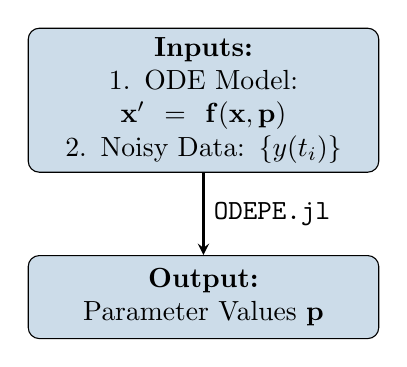
\begin{tikzpicture}[node distance=2.5cm, auto]
                \node[block] (inputs) {
                    \textbf{Inputs:} \\
                    1. ODE Model: $\mathbf{x}' = \mathbf{f}(\mathbf{x}, \mathbf{p})$ \\
                    2. Noisy Data: $\{y(t_i)\}$
                };
                \node[block, below of=inputs] (output) {
                    \textbf{Output:} \\
                    Parameter Values $\mathbf{p}$
                };

                \draw[arrow] (inputs) -- node[midway, right] {\texttt{ODEPE.jl}} (output);
            \end{tikzpicture}
        \end{column}
    \end{columns}
\end{frame}

% Slide 3: A Walkthrough of the Method (1/2)
\begin{frame}[fragile]{A Walkthrough of the Method (1/2)}
    \begin{block}{Example: $x' = a^2x^2 + b$, with output $y = x^2+x$}
    \footnotesize
    \begin{enumerate}
        \item \textbf{Differentiate System Symbolically:}\pause Relate parameters to higher-order derivatives of outputs ($y, y', y'', \dots$).
        \[
        \begin{aligned}
             y' &= (2x+1)x' \\
             y'' &= 2(x')^2 + (2x+1)x''
        \end{aligned}
        \quad
        \text{where}
        \quad
        \begin{aligned}
            x' &= a^2x^2+b \\
            x'' &= 2a^2xx'
        \end{aligned}
        \]
        \item \textbf{Approximate Derivatives from Data:}\pause At a time $t_i$, compute numerical values for $y(t_i), y'(t_i), \ldots$ from measurements. This is the critical step where GPR is used.
    \end{enumerate}
    \end{block}
\end{frame}

% Slide 4: A Walkthrough of the Method (2/2)
\begin{frame}{A Walkthrough of the Method (2/2)}
    \begin{block}{Example: $x' = a^2x^2 + b$, with output $y = x^2+x$}
    \footnotesize
    \begin{enumerate}
        \setcounter{enumi}{2} % Continue numbering
        \item \textbf{Form Polynomial System:}\pause Substitute numerical derivative values into the symbolic equations to create a polynomial system in the parameters and states.
        \item \textbf{Solve:}\pause Use a numerical polynomial solver to find all sets of solutions for the parameters ($a, b$) and states ($x(t_i)$).
        \item \textbf{Filter \& Validate:}\pause Use forward simulation to find the best-fitting parameter set.
    \end{enumerate}
    \end{block}
\end{frame}


% Slide 5: The Challenge
\begin{frame}{The Challenge: Real-World Data is Noisy}
    \begin{columns}[T]
        \begin{column}{0.5\textwidth}
            \begin{block}{The Problem}
                The original method, based on AAA baryrational interpolation, is extremely accurate on clean data but fails catastrophically with noise. Interpolation overfits, leading to unstable derivatives.
            \end{block}
        \end{column}
        \begin{column}{0.5\textwidth}
            \begin{figure}
                \includegraphics[width=\textwidth]{"Robust_Algebraic_Parameter_Estimation_via_Gaussian_Process_Regression/gpr_vs_aaa_comparison.pdf"}
                \caption{Interpolation vs. Regression}
            \end{figure}
        \end{column}
    \end{columns}
\end{frame}

% Slide 6: The Solution
\begin{frame}{The Solution: Taming Noise with Gaussian Process Regression}
    \begin{block}{Why Gaussian Process Regression (GPR)?}
    \normalsize
    GPR defines a \textit{prior distribution over functions} and updates it based on the data.
    \begin{itemize}
        \item \textbf{Principled Smoothing:} A smoothness assumption is encoded in the prior via a kernel function (e.g., RBF).
        \item \textbf{Noise Modeling:} GPR explicitly models measurement noise, learning the noise level from the data itself.
        \item \textbf{Analytic Derivatives:} The posterior mean function is smooth and can be differentiated reliably.
    \end{itemize}
    \end{block}
    
    \begin{alertblock}{The Result}
        \centering
        \Large
        Robust and accurate derivative estimation, even with noisy data.
    \end{alertblock}
\end{frame}

% Slide 7: The Results
\begin{frame}{The Results: Robust and Accurate}
    \begin{block}{Benchmark on Nonlinear Systems}
        \centering
        \tiny
        \input{"Robust_Algebraic_Parameter_Estimation_via_Gaussian_Process_Regression/summary_table.tex"}
    \end{block}
    
    \begin{alertblock}{Key Takeaway}
        \centering
        \Large
        The GPR-enhanced method is robust to noise, making it practical for real-world applications.
    \end{alertblock}
\end{frame}

% Slide 7: Why Julia?
\begin{frame}{Why Julia?}
    \Large
    Julia is the perfect language for this kind of work!
    
    \begin{itemize}
        \item \large\textbf{Symbolic Manipulation:} Symbolics.jl
        \item \large\textbf{Numerical Methods:} DifferentialEquations.jl, GaussianProcesses.jl, Groebner.jl, HomotopyContinuation.jl 
        \item \large\textbf{High Performance:} Fast enough for complex systems.
        \item \large\textbf{Composable:} Easy to combine different tools and packages.
    \end{itemize}
\end{frame}

% Slide 8: Get Involved!
\begin{frame}{Get Involved!}
    \begin{center}
        \Large
        \texttt{github.com/orebas/ODEParameterEstimation}
        
        \vspace{2em}
        
        \large
        (Formerly known as ParameterEstimation.jl)
        
        \vspace{1em}
        
        \normalsize
        Oren Bassik \\
        obassik@gradcenter.cuny.edu
    \end{center}
\end{frame}

% Slide 9: Q&A
\begin{frame}
    \begin{center}
        \huge Thank You
        \vspace{2em}
        
        \Large Questions?
    \end{center}
\end{frame}

\end{document} 